\chapter{Numerical Studies}\label{chapter:numerical_study}
Having discussed how the NSE were simplified, discretized, and implemented, in this section we test and validate the implementation.
To this end we discuss the results of the unit tests from Section~\ref{sec:testing} by looking at the numerical errors made by the differential operators and integrators.
Thereafter we analyze the implementations of the non-hydrostatic NSE discussed in Section~\ref{sec:non_hydrostatic}.

\section{Validation by Analyzing Numerical Errors}
%In this section we discuss the results of the tests performed in Section~\ref{sec:testing}.

% analysis of errors
\subsection{Differential Operators}\label{sec:numeric_diff_ops}
To test the differential operators, the function $f(x)=\sin(20\pi (x-e))$ with derivative $\frac{df}{dx}=20\pi\cos(20\pi (x-e))$ was used on the domain $[0;1]$.
The offset of $e$ was included in order to avoid random perfect results.
For example. if maxima, minima and zero crossings happen to be located exactly at sample point, even a simple central difference would result in no error.
With an offset of an irrational number, such as $e$, this is improbable.

To test the different methods of calculating the derivative numerically, we sampled the domain at resolutions ranging from $5$ to $20\cdot 10^7$ samples which were spread equidistantly across the domain.
\begin{figure}[!h]
	\makebox[\textwidth]{ 
  		 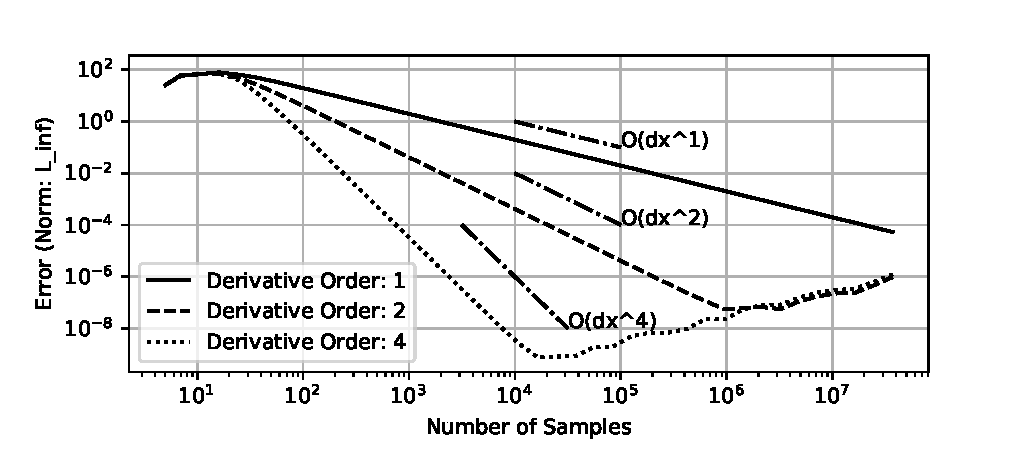
\includegraphics[width=1.1\textwidth]{figures/derivative_error.pdf}}
    \caption{Plot of error of finite difference operators over number of samples;
    the lines are parallel to the expected error order lines, meaning the test was successful.}
    \label{fig:derivative_error}
\end{figure}
\begin{figure}[!h]
	\makebox[\textwidth]{ 
  		 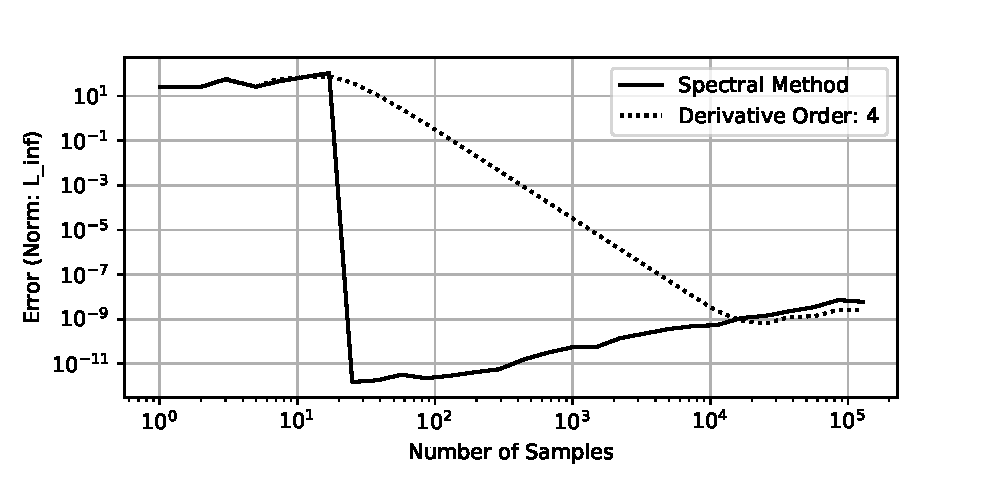
\includegraphics[width=1.1\textwidth]{figures/fft_error.pdf}}
    \caption{Plot of error of spectral derivative operator over number of samples;
    as expected the error drops significantly as soon as the Nyquist sampling rate (20 samples) is reached.}
    \label{fig:fft_error}
\end{figure}
We first look at the implementation of the finite differences.
If their implementation is correct, we expect the error [\texttt{finite\_difference(x)}$-\frac{df}{dx}$] to drop with increasing resolution.
More specifically for a finite difference operator of order $n$, when increasing the number of samples by a factor of $a$ we expect a decrease in error by a factor of $a^{-n}$.
The positive result of the test can be seen in Fig.~\ref{fig:derivative_error}.

We can also see that above a certain spatial resolution, the error increases again which is due to numerical errors.
The root of these errors is the division of a very small number in the denominator by the small number $\Delta x$ which is inversely proportional to the resolution.
This division of small numbers is not well-supported by floating point numbers, and for that reason errors increase above a certain spatial resolution.

Concerning the spectral derivative, we would expect that the error drops down to machine precision as soon as the Nyquist sampling rate is reached.
The Nyquist sampling rate is twice the highest frequency occurring in the signal whose derivative is to be calculated.
In this case the highest frequency is $10$, because the argument of $\sin$ was $2\pi\cdot 10$, meaning the Nyquist sampling rate is $20$.
The fact this theoretical result can be observed in practice (Fig.~\ref{fig:fft_error}), is a strong indication that the implementation is correct.


\FloatBarrier

%Test-Function: $\sin(20\pi (x-e))$ on domain $[0;1]$, with resolutions from 5 to $20\cdot 10^7 $
%Actual result is $20\pi\cos(20\pi (x-e))$\\
%show how the error-order is influenced by grid-size.\\
%grid size far larger than features to be measured => inaccuracy\\
%grid size a little bit smaller than features to be measured => change in accuracy according to error-order of implemented operator\\
%grid size too small for machine precision => loss of accuracy

\subsection{Integrators}
\subsubsection{Runge-Kutta-Integrators}
As described in Section~\ref{sec:testing}, we tested the integrators by comparing the results to analytic solution of differential equations.
Specifically, we first tested against three types of differential equations, whose solutions are known analytically.
The first one was time-invariant and had only one variable, i.e. no spatial resolution.
The second one introduced time-variance, while the third one added spatial resolution.
In each of the tests, using a Runge-Kutta integrator of order $n$ we expected that decreasing the time step size by a factor of $a$ would decrease the error by a factor of $a^n$.

\begin{figure}[!h]
	\makebox[\textwidth]{ 
  		 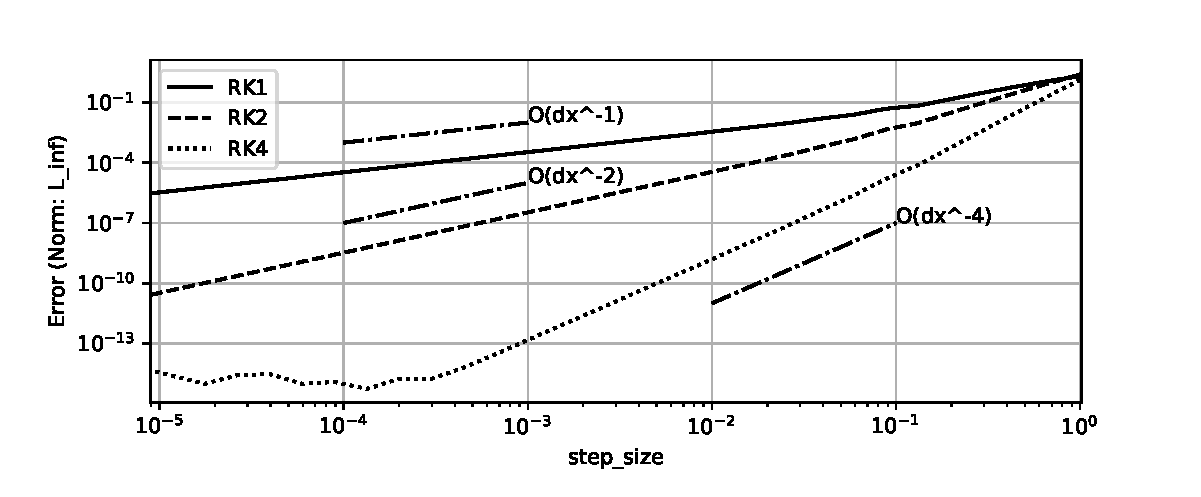
\includegraphics[width=1.2\textwidth]{figures/RK_error_y'=-3y.pdf}}
    \caption{Error of RK-methods on time-invariant, single variable differential equation}
    \label{fig:RK_error_y'=-3y}
\end{figure}
\begin{figure}[!h]
	\makebox[\textwidth]{ 
  		 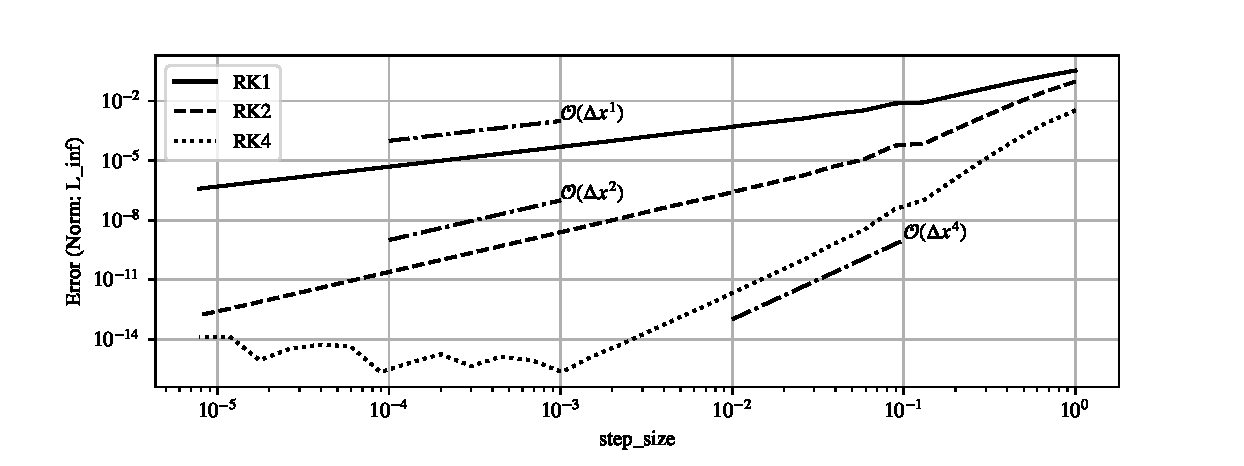
\includegraphics[width=1.3\textwidth]{figures/RK_error_y'=tdiv(t_t+1).pdf}}
    \caption{Error of RK-methods on time-variant, single variable differential equation}
    \label{fig:RK_error_y'=tdiv(t_t+1)}
\end{figure}

\paragraph*{Time-Invariant, Single Variable}
The differential equation is $\frac{dx}{dt}=-3x$ which has the solution $x(t)=x_0e^{-3t}$.
The result of the experiment can be seen in Fig.~\ref{fig:RK_error_y'=-3y}.

\paragraph*{Time-Variant, Single Variable}
The differential equation is $\frac{dx}{dt}=\frac{t}{t^2+1}$ which has the solution $x(t)=x_0 + 0.5\text{ln}(t^2+1)$.
The result of the experiment can be seen in Fig.~\ref{fig:RK_error_y'=tdiv(t_t+1)}.

\paragraph*{Time-Invariant, Multiple Spatially Distributed Variables}
The differential equation is the wave equation with periodic boundary conditions.
With $c$ being the wave propagation speed, the equation system can be written as follows:
\begin{align*}
\frac{du}{dt}&=\frac{dv}{dx}\\
\frac{dv}{dt}&=c^2\frac{du}{dx}
\end{align*}
If $u(x,t=0)=f(x)$ (with $f$ being periodic) describes the initial state of $u$, then according to d'Alembert the solution is:
\begin{align*}
u(x,t)&=\frac{1}{2}(f(x+ct)+f(x-ct))\\
\Rightarrow v(x)&=\int \frac{du}{dt} dx = \frac{c}{2}(f(x+ct)-f(x-ct))
\end{align*}
The result of the experiment can be seen in Fig.~\ref{fig:wave_order_line}.

\begin{figure}[!h]
	\makebox[\textwidth]{ 
  		 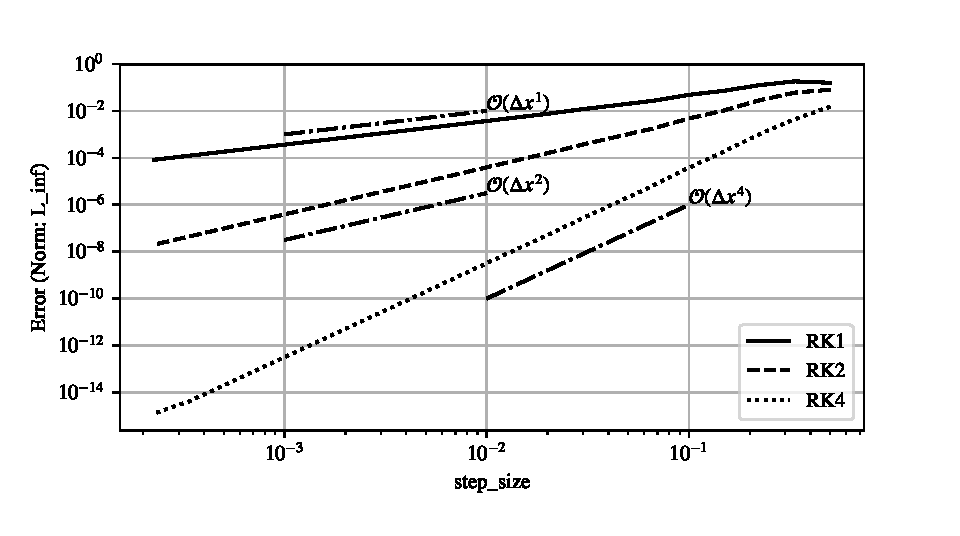
\includegraphics[trim={0 0.75cm 0 0.9cm},clip,width=1.0\textwidth]{figures/wave_order_line.pdf}}
    \caption{Error of RK-methods on periodic wave equation}
    \label{fig:wave_order_line}
\end{figure}
\begin{figure}[!h]
	\makebox[\textwidth]{ 
  		 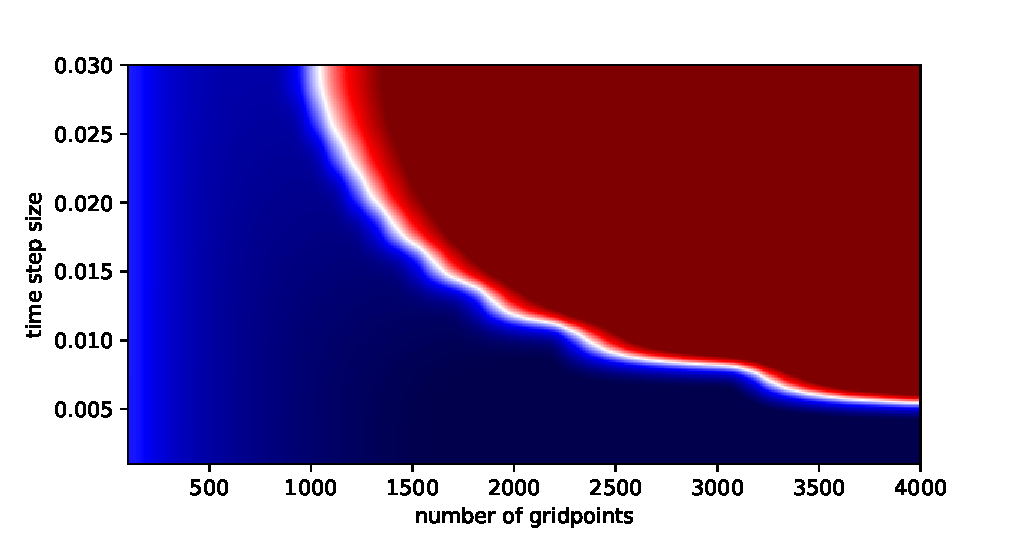
\includegraphics[width=1.175\textwidth]{figures/heatmap_wave_eq_step_size_numgridpoints.pdf}}
    \caption{Heatmap of ln(Error) for wave equation over different spatial and temporal resolutions;
    the white stripe represents the area where the log-error is 0, i.e. the actual error is 1.
In the red and the blue areas the log-error is positive (up to $150$) and negative (down to $-20$), respectively.}
    \label{fig:heatmap_wave_eq_step_size_numgridpoints}
%	\small

\end{figure}


Interestingly, spatial resolution and temporal resolution are intertwined.
If a very high spatial resolution (a lot of samples) is chosen, one also must choose a high temporal resolution (small time steps).
This can be seen when plotting a heatmap of the error made with the RK4-integrator over different spatial and temporal resolutions.
This phenomenon can be seen in Fig.~\ref{fig:heatmap_wave_eq_step_size_numgridpoints}.
Roughly speaking, in order to keep the error from diverging, an inverse proportion between spatial resolution and time step size should be kept.
For example, when doubling the spatial resolution, one should at least halve the time step size, in order to stay stable.


%$frac{dx}{dt}=\frac{t}{t^2+1}$ which has the solution $x_0 + 0.5\text{ln}(t^2+1)$.



%a time-invariant differential equation with only one variable (i.e. no spatial resolution), then a time-variant differential equation with no spatial resolution, and finally against a differential.
%First off, to verify the implementation, the RK-Integrators were used to solve a differential equation without any spatial resolution, but with temporal variance.
%$\frac{dx}{dt}=\frac{t}{t^2+1}$
%with solution $x_0 + 0.5\text{ln}(t^2+1)$.

%explain how time-step-size and grid-size must change together, and show trough examples how accuracy changes depending on the choice of these two parameters (maybe a heatmap with x-axis = time-step-size, y-axis=grid-size, color=accuracy after simulation time T?)
%\subsubsection{Exponential Integrators}
%showcase how accuracy stays constant independent of time-step-size (for linear systems)\\
%give a small example of simulating a non-linear system by linearization around the current state


\section{Study of Errors in Implementation of NSE}
In this section we analyze the two implementations of the NSE.
As no single standardized benchmarking system for testing the vertical dimension of the non-hydrostatic NSE-equations in isolation exists, complete verification of the implementation is not possible.
Instead, we considered four tests:
\begin{itemize}
\item comparison with a stationary solution
\item comparison of stationary solution with real world measurements
\item energy conservation
\item comparison of the two implementations to one another
\end{itemize}
Due to the nature of the non-hydrostatic NSE, we cannot test for mass conservation, because mass is always preserved according to Eq.~\ref{eq_mass_conservation}.

\subsection{Comparison with Stationary Solution}
We first test the implementation by cross-checking it with the stationary solution.
This means that the system's state must stay constant in case the starting condition is a stationary solution of the non-hydrostatic NSE.
To find a stationary solution for the non-hydrostatic NSE, we set all time-derivatives to zero:
\begin{align}
\frac{\partial w}{\partial t} =0&= -g\left(1 - \frac{\partial p}{\partial s}\left(\frac{\partial \pi}{\partial s}\right)^{-1}\right)\label{stat_dw_dt} \\
\frac{\partial \text{ln}p}{\partial t}=0 &= \frac{g}{1- \frac{R}{C_p}} \frac{p}{RT}\left(\frac{\partial \pi}{\partial s}\right)^{-1} \frac{\partial w}{\partial s}\label{stat_dlnp_dt}\\
\frac{\partial T}{\partial t} =0&= \frac{RT}{C_p}\frac{\partial \text{ln}p}{\partial t}\label{stat_dT_dt}
\end{align}
The first equation Eq.~\ref{stat_dw_dt} yields the following identity for pressure:
\begin{align*}
\frac{\partial p}{\partial s}=\left(\frac{\partial \pi}{\partial s}\right)\\
\Rightarrow p(s)=\pi (s) + p_0
\end{align*}
The second equation Eq.~\ref{stat_dlnp_dt} requires one of the elements in the denominator to equal zero.
As neither $g$, $p$, nor $\left(\frac{\partial \pi}{\partial s}\right)^{-1}$ can be zero, the only possible option is that $\frac{\partial w}{\partial s}=0$, i.e. $w(s)=w_0 \forall s$.
Due to the boundary conditions, at the bottom of the atmosphere $w(s=1)=0$, so $w(s)=w_0 \forall s$.

The last equation Eq.~\ref{stat_dT_dt} yields no information, because the right hand side is already zero, due to $\frac{\partial \text{ln}p}{\partial t}=0$.
This means $T$ can be chosen freely, e.g. $T=273K$.
Using this stationary solution to define the initial state of the system, the integrator is expected not to change the system state.
This is reflected by both implementations as can be seen in Fig.~\ref{fig:lorenz_stat_err}, where the magnitude of the error is never greater than $10^{-8}$.

\begin{figure}[!h]
%	\makebox[\textwidth]{ 
%  		 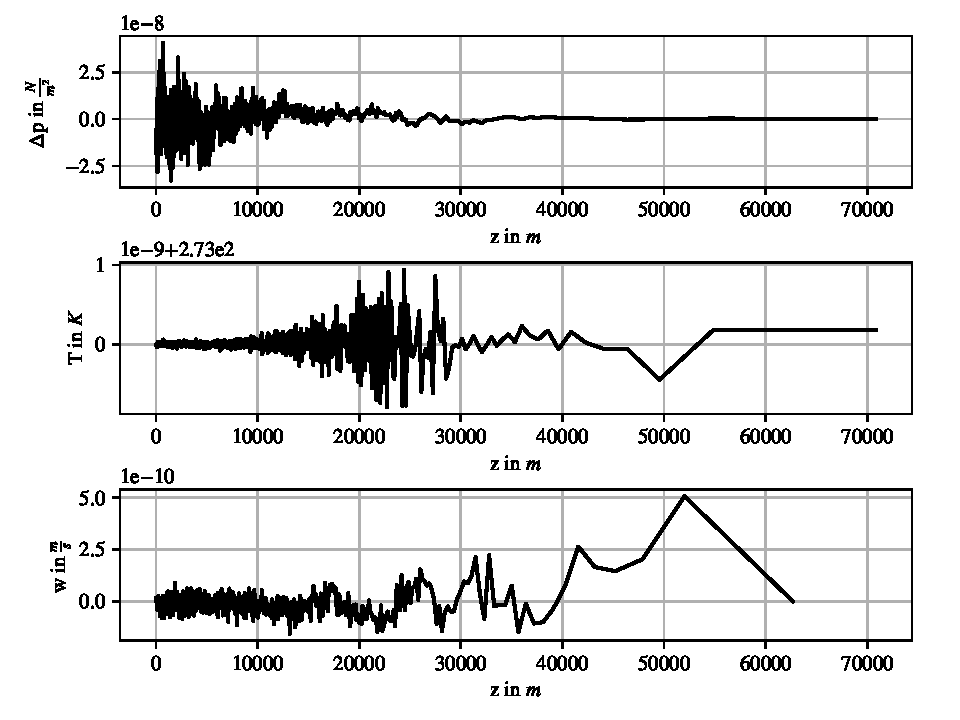
\includegraphics[width=1.0\textwidth]{figures/lorenz_240s_stat.pdf}}
    \makebox[\textwidth]{ 
  		 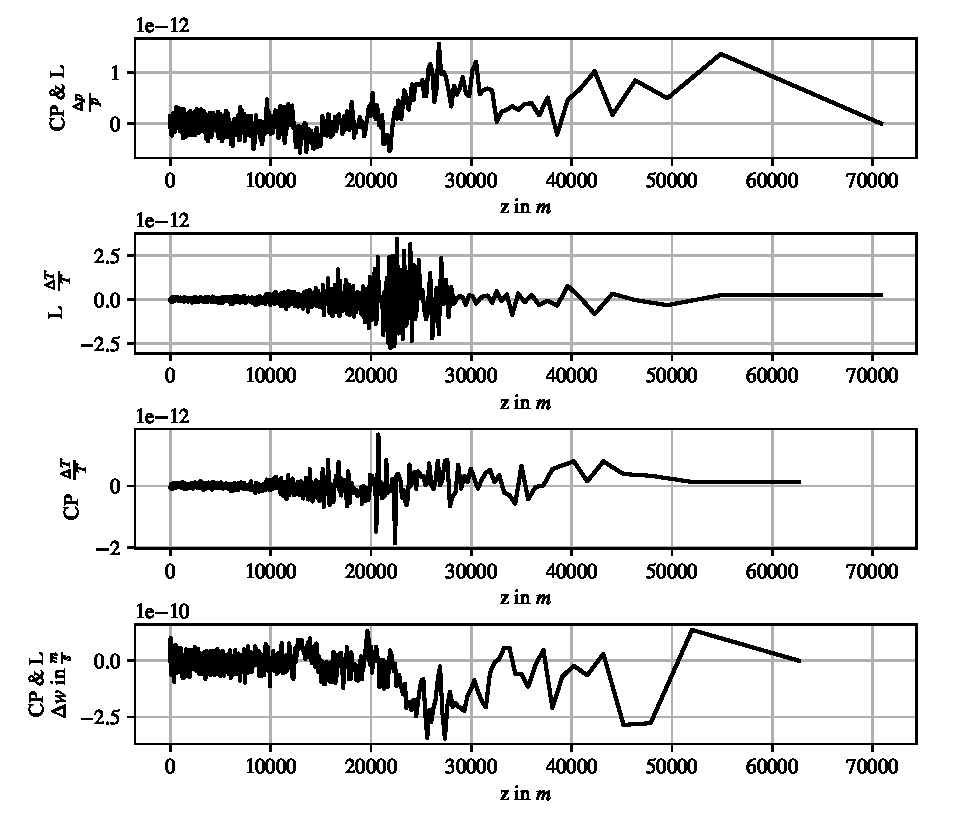
\includegraphics[width=1.0\textwidth]{figures/l_cp_240s_error.pdf}}
    \caption{Relative Error (deviation from stationary solution) with RK4, time-step-size $2.5ms$, and $1000$ grid points, after $240s$ of simulation time on Lorenz grid (L) and Charney-Phillips-grid (CP);
    the plots for $\frac{\Delta \text{ln}p}{p}$ and $\Delta w$ for both simulations were essentially identical, so both were only plotted once.}

    %\caption{Error (deviation from stationary solution) with RK4, time-step-size $2.5ms$, and $1000$ grid points, after $240s$ of simulation time on Lorenz grid (the corresponding diagram \ref{fig:cp_stat_err} for the Charney-Phillips-grid is nearly identical and can be found in appendix \ref{sec:stationary_cp_error})}
    \label{fig:lorenz_stat_err}
    
\end{figure}

\subsection{Comparison with Real World Measurements}
Another method to test the implementation is a comparison with measurements from the real world.
First, we can compare the distribution of density $\rho=\frac{p}{RT}$ in the stationary case to real world measurements of the atmosphere made by NASA~\cite{larson1963stratosphere}.
For the simulation we assumed that pressure at the bottom of the system was $\pi_{bottom}=1atm=101325 Pa$, and $T=273K$.
Additionally, it was assumed that $\pi (s) = s\cdot\pi_{bottom}$
In Fig.~\ref{fig:cmp_nasa} it can be seen that the calculated result closely mirrors reality.


\begin{figure}[!h]
	\makebox[\textwidth]{ 
  		 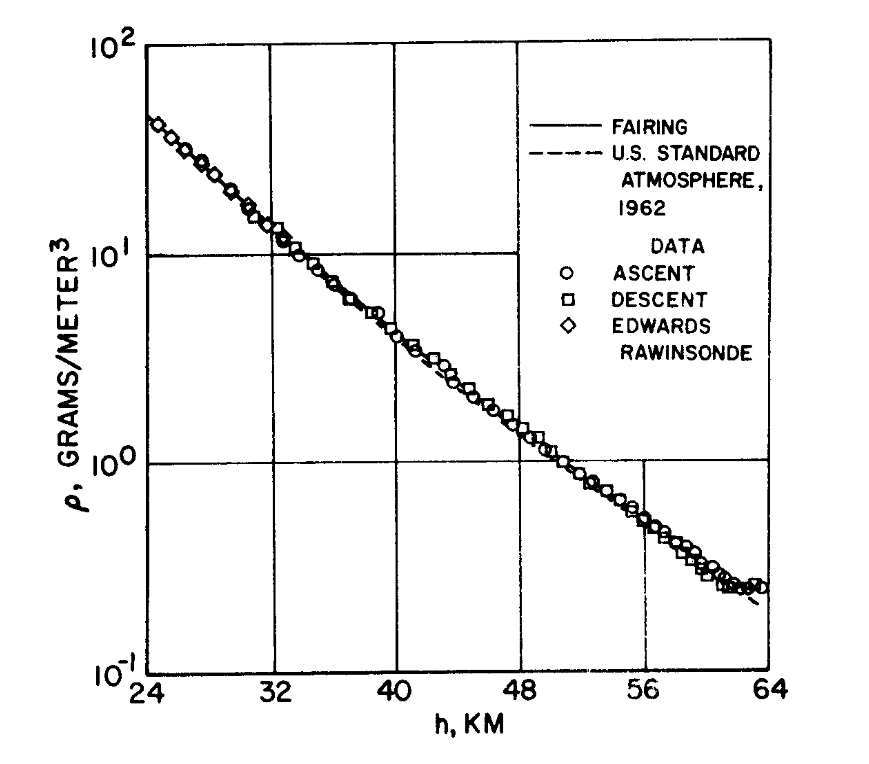
\includegraphics[width=0.5\textwidth]{figures/height_density_nasa.png}
  		 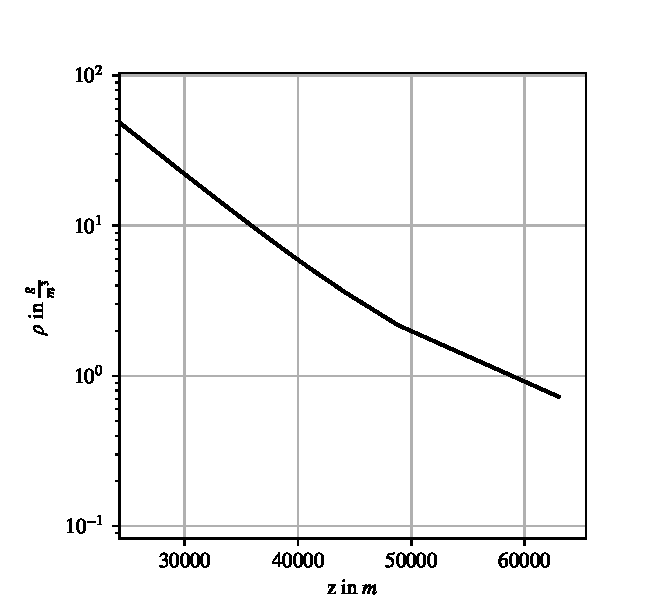
\includegraphics[width=0.5\textwidth]{figures/height_density.pdf}}
    \caption{Comparison of real world measurements from NASA~\cite{larson1963stratosphere} with simulated results.}
    \label{fig:cmp_nasa}
\end{figure}

The second comparison with real world measurements is the speed of sound.
The speed of sound is essentially the speed at which a region of increased pressure travels, i.e. the wave speed of the system.
To measure wave speed an appropriate starting condition containing a region of increased pressure must be defined.
Then the location of this bump must be measured over time.
From the trace of time and location of the bump, its speed can be calculated by taking the derivative of location over time.

The result of such an experiment can be seen in Fig.~\ref{fig:sound_speed}, namely that the speed of sound in the simulation ranges between $331\frac{m}{s}$ and $341\frac{m}{s}$.
This is close to the actual speed of sound at sea level around $331\frac{m}{s}$ according to~\cite{hardy1942velocity}.

\begin{figure}[!h]
	\makebox[\textwidth]{ 
  		 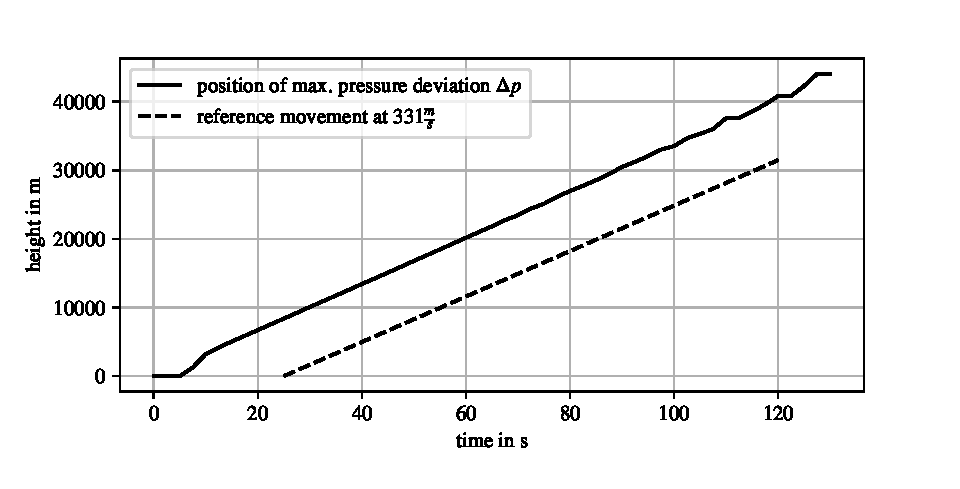
\includegraphics[width=1.0\textwidth]{figures/sound_speed.pdf}}
    \caption{Graph of location over time of (a) a region of increased pressure; (b) a reference object moving at the speed of sound ($331\frac{m}{s}$);
    the simulation was run with $1000$ grid points and a time step size of $2.5ms$ on a Lorenz-grid. Simulations on Charney-Phillips-grids yield similar results.}
    \label{fig:sound_speed}
\end{figure}

For the experiment, the starting condition was chosen as follows: $T=273K$, $w=0$.
For $p$ we began with the stationary solution as a baseline, i.e. $p(s)=\pi (s)$.
Then we added a Gaussian bell~curve of magnitude $1\frac{N}{m^2}$ with its maximum at the bottom $s=1$ onto this configuration.
Inserting the Gaussian bump at any location other than the boundary of the domain would result in two regions of increased pressure traveling across the atmosphere.
This would make measurements within the simulation more difficult.

Note that this is one of the key differences between simulation with the hydrostatic NSE versus with the non-hydrostatic NSE.
According to Coiffier, usage of the hydrostatic NSE ``eliminates sound waves because of the hydrostatic relation which has a \emph{filtering} effect on them''~\cite{coiffier2011fundamentals}.

\subsection{Energy Conservation}\label{sec:energy_conservation_test}
The third way of testing the implementation is testing the hypothesis of energy conservation.
As the choice of boundary conditions dictates that energy in the system must stay constant, every simulation of the non-hydrostatic NSE should have the same property.
That is, every system state produced by the simulation should have the same energy as the starting condition.

To this end we employ the formula for calculating the total energy in the system per area~\ref{eq_energy}:
\begin{align*}
E'=\int_{s_{top}}^{s_{bottom}} \frac{1}{g}(C_vT+\frac{1}{2}w^2 + gz(s)) \left( \frac{\partial \pi}{\partial s} \right) ds
\end{align*}
When assuming energy to stay constant over time, it makes sense to take the energy contained in the system at the beginning as a baseline.
This way, by subtracting the baseline energy from the energy calculated at some later time during simulation, we can track the error over time.

Of course, in order for it to be possible for an error to appear, the system must change over time, i.e. not be stationary.
Other than that any starting condition may be chosen.
For the following simulations, the starting conditions were as follows: $T=273K$, $w=0$.
For $p$ the stationary solution was taken as a baseline, i.e. $p(s)=\pi (s)=s\cdot 101325\frac{N}{m^2}$.
Then a Gaussian bell curve of magnitude $0.1\frac{N}{m^2}$ with its maximum at $z=35km$ was added onto this configuration.

The results of this for both the Lorenz-grid and the Charney-Phillips-grid can be seen in Fig.~\ref{fig:energy_error}.
The baseline energy for both grids was nearly identical (down to the fifteenth digit) at $E'_0=2.814\cdot 10^9J$. %$2814147192.3283653J$.

\begin{figure}[!h]
	\makebox[\textwidth]{ 
  		 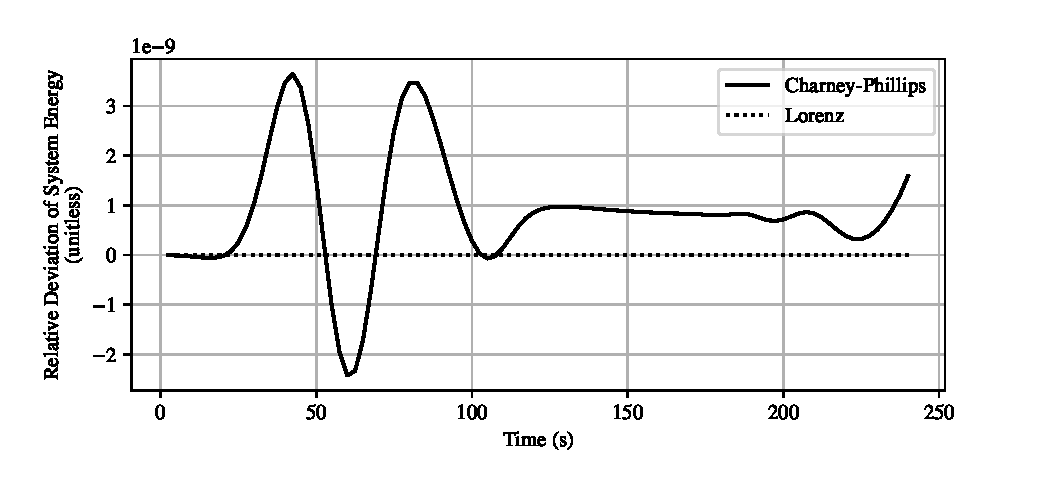
\includegraphics[width=1.0\textwidth]{figures/cp_energy_rel_error.pdf}}
  	\makebox[\textwidth]{
  		 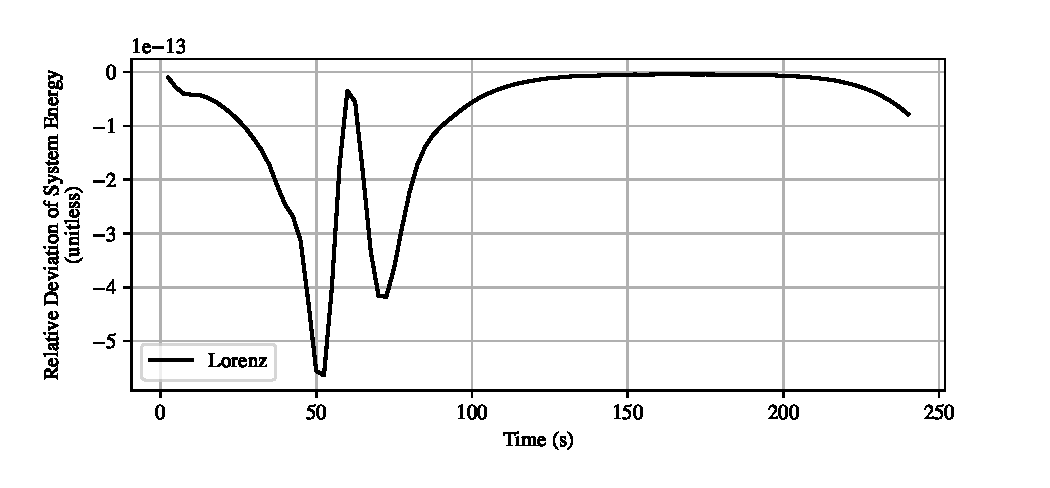
\includegraphics[width=1.0\textwidth]{figures/lorenz_energy_rel_error.pdf}}
    \caption{Relative energy deviation $\frac{E'(t)-E'_0}{E'_0}$ over time for Lorenz-Grid and Charney-Phillips-grid;
    both simulations were run with $1000$ grid points and a time step size of $2.5ms$.}
    \label{fig:energy_error}
\end{figure}

It can be seen that usage of the Lorenz-grid leads to lower errors in energy conservation, than usage of the Charney-Phillips-grid.
This is in line with the design goal of energy conservation Lorenz had in mind when designing his grid~\cite{lorenz1960energy}.

To explain the larger error when employing the Charney-Phillips-grid, one must look at the composition of energy.
Recall that energy in the atmospheric system can be split up into three components: internal energy, kinetic energy, and geopotential energy.

\begin{figure}[!h]
	\makebox[\textwidth]{ 
  		 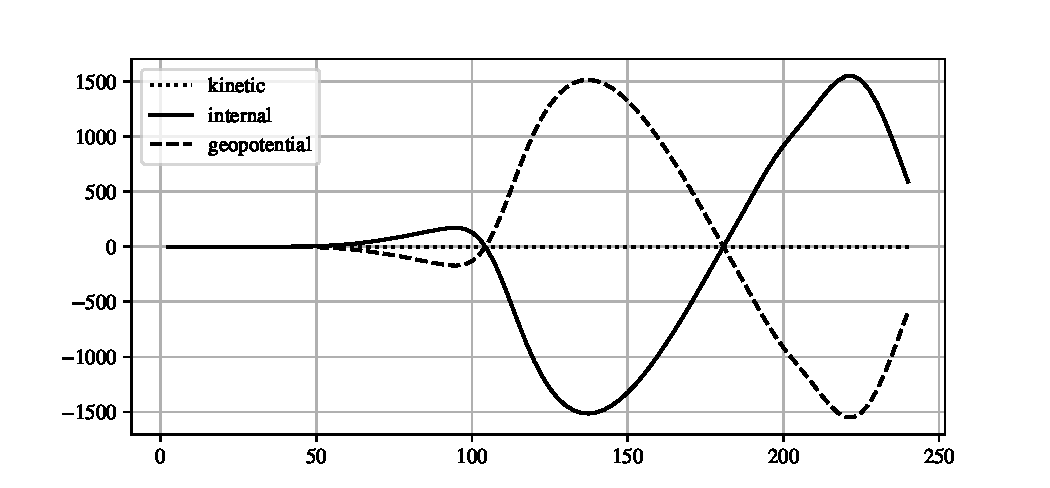
\includegraphics[width=1.0\textwidth]{figures/cp_energy_split.pdf}}
    \caption{Deviation of each component of energy over time for Charney-Phillips-grid;
    the simulation was run with $1000$ grid points and a time step size of $2.5ms$.
    }
    \label{fig:cp_energy_split}
\end{figure}
\noindent
When plotting the individual deviations for each component, as is done in Fig.~\ref{fig:cp_energy_split}, one can see that the kinetic energy deviation is rather negligible at around $3\cdot10^{-3}J$.
Instead the increased energy deviation for the Charney-Phillips-grid must originate from an asymmetry between the deviation of internal and geopotential energy.
It appears that this asymmetry is inherently rooted in the averaging operation necessary to calculate the time-derivative for temperature $T$ numerically.

Looking further at the averaging operation, we recall the prognostic equation for $T$:
\begin{align*}
\frac{\partial T}{\partial t} &= \frac{RT}{C_p}\frac{\partial \text{ln}p}{\partial t}\\
&=\frac{gp}{C_p-R}\left(\frac{\partial \pi}{\partial s}\right)^{-1} \frac{\partial w}{\partial s}
\end{align*}

We see that $T$ either depends on $\frac{\partial \text{ln}p}{\partial t}$, or $p$ (when substituting in the prognostic equation for $\frac{\partial \text{ln}p}{\partial t}$).
For the Charney-Phillips-grid, both of these variables are sampled on the offset grid, meaning that in order to calculate $\frac{\partial T}{\partial t}$, an averaging operator must be applied.
Taking an average is not especially accurate.
This explanation supports the interpretation that there is no implementation error.

In light of this, when conservation of energy is essential, the Lorenz grid should be preferred when simulating the non-hydrostatic NSE.

\subsection{Comparison of the two Implementations}
Finally, we tested the two implementations by comparing the simulation outputs after a certain amount of elapsed time.
For purposes of this test, we initialized both implementations with identical starting conditions.
Just like in the previous section, any starting condition can be chosen.
For simplicity's sake, we employ the same starting condition as in the previous Section~\ref{sec:energy_conservation_test}.

Using said starting condition, we ran both simulations for $240s$ of simulation time, with a spatial resolution of $1000$ grid points, and a temporal resolution of $2.5ms$.
The result of the two simulations on the different grids can be seen in Fig.~\ref{fig:simulations}.

The similar appearance of the separate simulation results for pressure deviation $\Delta p$ and vertical wind speed $w$ is no optical illusion.
It can also be verified numerically:
When taking the difference between the two simulation results, the largest absolute difference\footnote{Also known as the $L_\infty$-norm} for $\Delta p$ is $8.71\cdot 10^{-11}$, and the largest absolute difference for $w$ is $9.32\cdot 10^{-9}$.
We did not determine the difference for $T$, because the two $T$-grids are offset to one another by definition of the Charney-Phillips and Lorenz grids, so any comparison would require inaccurate averaging operations.

The minuscule difference of $\Delta p$ and $w$ between implementations reaffirms the assumption made in Section~\ref{sec:energy_conservation_test} that the error in energy conservation for the Charney-Phillips grid must stem from inaccuracies in $T$.

In summary, both implementations pass all tests.

\begin{figure}[!h]
	\makebox[\textwidth]{ 
  		 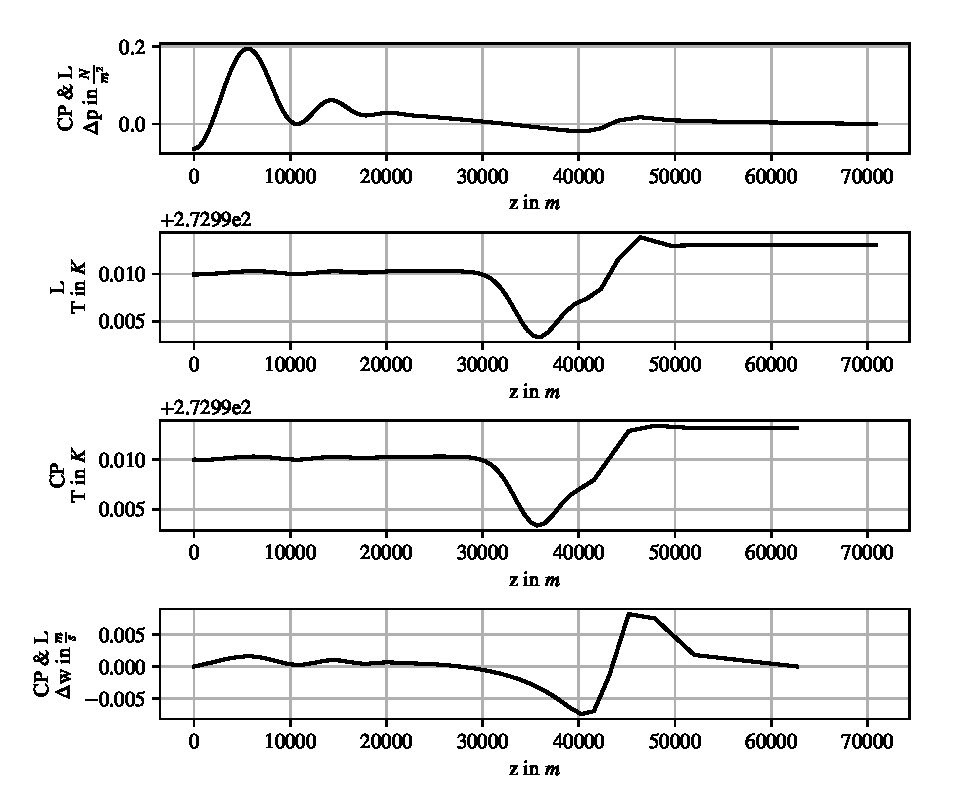
\includegraphics[width=1.1\textwidth]{figures/l_cp_240s_bump.pdf}}
%	\makebox[\textwidth]{ 
 % 		 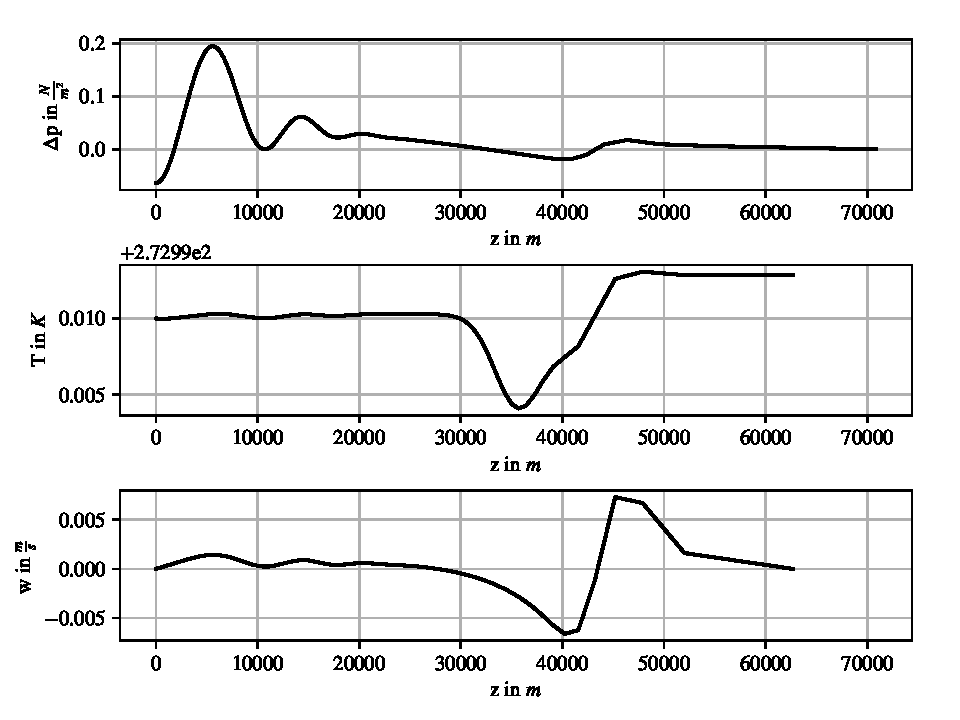
\includegraphics[width=0.8\textwidth]{figures/cp_240s_bump.pdf}}  		 
  %	\makebox[\textwidth]{
  	%	 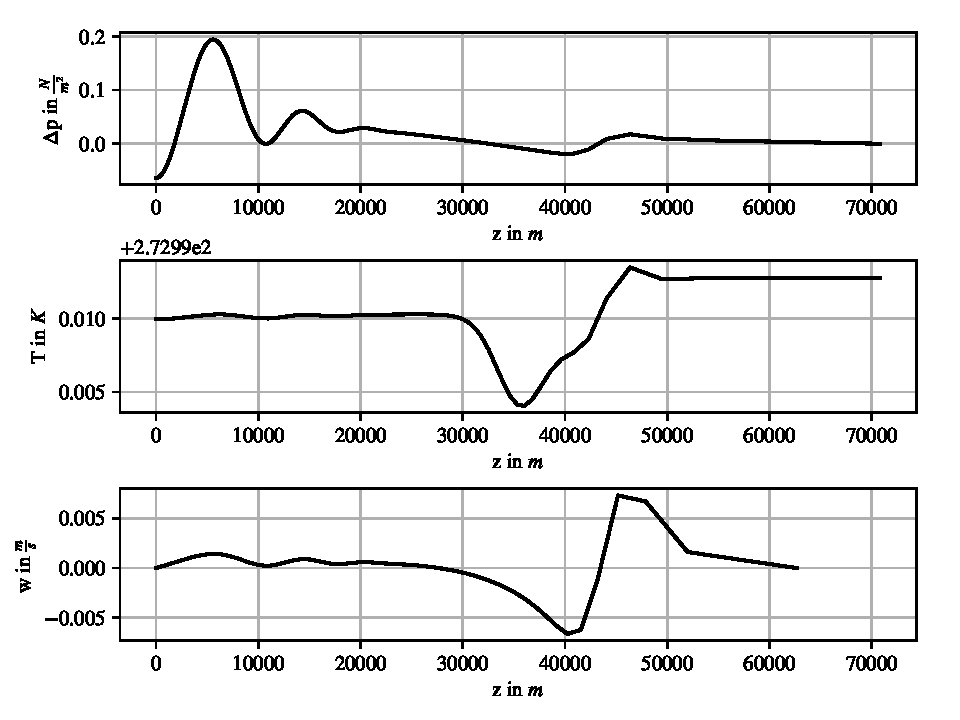
\includegraphics[width=0.8\textwidth]{figures/lorenz_240s_bump.pdf}}
    \caption{Simulation results for Charney-Phillips grid (CP), and the Lorenz grid (L);
    the plots for $\text{ln}p$ and $\Delta w$ for both simulations were nearly identical, so both were only plotted once.
Both simulations were run for $240s$ with $1000$ grid points and a time step size of $2.5ms$.}
    \label{fig:simulations}
    \small

\end{figure}

